% GNUPLOT: LaTeX picture with Postscript
\begingroup
  \makeatletter
  \providecommand\color[2][]{%
    \GenericError{(gnuplot) \space\space\space\@spaces}{%
      Package color not loaded in conjunction with
      terminal option `colourtext'%
    }{See the gnuplot documentation for explanation.%
    }{Either use 'blacktext' in gnuplot or load the package
      color.sty in LaTeX.}%
    \renewcommand\color[2][]{}%
  }%
  \providecommand\includegraphics[2][]{%
    \GenericError{(gnuplot) \space\space\space\@spaces}{%
      Package graphicx or graphics not loaded%
    }{See the gnuplot documentation for explanation.%
    }{The gnuplot epslatex terminal needs graphicx.sty or graphics.sty.}%
    \renewcommand\includegraphics[2][]{}%
  }%
  \providecommand\rotatebox[2]{#2}%
  \@ifundefined{ifGPcolor}{%
    \newif\ifGPcolor
    \GPcolorfalse
  }{}%
  \@ifundefined{ifGPblacktext}{%
    \newif\ifGPblacktext
    \GPblacktexttrue
  }{}%
  % define a \g@addto@macro without @ in the name:
  \let\gplgaddtomacro\g@addto@macro
  % define empty templates for all commands taking text:
  \gdef\gplfronttext{}%
  \gdef\gplfronttext{}%
  \makeatother
  \ifGPblacktext
    % no textcolor at all
    \def\colorrgb#1{}%
    \def\colorgray#1{}%
  \else
    % gray or color?
    \ifGPcolor
      \def\colorrgb#1{\color[rgb]{#1}}%
      \def\colorgray#1{\color[gray]{#1}}%
      \expandafter\def\csname LTw\endcsname{\color{white}}%
      \expandafter\def\csname LTb\endcsname{\color{black}}%
      \expandafter\def\csname LTa\endcsname{\color{black}}%
      \expandafter\def\csname LT0\endcsname{\color[rgb]{1,0,0}}%
      \expandafter\def\csname LT1\endcsname{\color[rgb]{0,1,0}}%
      \expandafter\def\csname LT2\endcsname{\color[rgb]{0,0,1}}%
      \expandafter\def\csname LT3\endcsname{\color[rgb]{1,0,1}}%
      \expandafter\def\csname LT4\endcsname{\color[rgb]{0,1,1}}%
      \expandafter\def\csname LT5\endcsname{\color[rgb]{1,1,0}}%
      \expandafter\def\csname LT6\endcsname{\color[rgb]{0,0,0}}%
      \expandafter\def\csname LT7\endcsname{\color[rgb]{1,0.3,0}}%
      \expandafter\def\csname LT8\endcsname{\color[rgb]{0.5,0.5,0.5}}%
    \else
      % gray
      \def\colorrgb#1{\color{black}}%
      \def\colorgray#1{\color[gray]{#1}}%
      \expandafter\def\csname LTw\endcsname{\color{white}}%
      \expandafter\def\csname LTb\endcsname{\color{black}}%
      \expandafter\def\csname LTa\endcsname{\color{black}}%
      \expandafter\def\csname LT0\endcsname{\color{black}}%
      \expandafter\def\csname LT1\endcsname{\color{black}}%
      \expandafter\def\csname LT2\endcsname{\color{black}}%
      \expandafter\def\csname LT3\endcsname{\color{black}}%
      \expandafter\def\csname LT4\endcsname{\color{black}}%
      \expandafter\def\csname LT5\endcsname{\color{black}}%
      \expandafter\def\csname LT6\endcsname{\color{black}}%
      \expandafter\def\csname LT7\endcsname{\color{black}}%
      \expandafter\def\csname LT8\endcsname{\color{black}}%
    \fi
  \fi
    \setlength{\unitlength}{0.0300bp}%
    \ifx\gptboxheight\undefined%
      \newlength{\gptboxheight}%
      \newlength{\gptboxwidth}%
      \newsavebox{\gptboxtext}%
    \fi%
    \setlength{\fboxrule}{0.5pt}%
    \setlength{\fboxsep}{1pt}%
\begin{picture}(8400.00,4000.00)%
    \gplgaddtomacro\gplfronttext{%
    }%
    \gplgaddtomacro\gplfronttext{%
      \colorrgb{0.15,0.15,0.15}%
      \put(114,1003){\makebox(0,0)[r]{\strut{}$0.05$}}%
      \colorrgb{0.15,0.15,0.15}%
      \put(114,1571){\makebox(0,0)[r]{\strut{}$0.10$}}%
      \colorrgb{0.15,0.15,0.15}%
      \put(114,2137){\makebox(0,0)[r]{\strut{}$0.15$}}%
      \colorrgb{0.15,0.15,0.15}%
      \put(114,2705){\makebox(0,0)[r]{\strut{}$0.20$}}%
      \colorrgb{0.15,0.15,0.15}%
      \put(114,3273){\makebox(0,0)[r]{\strut{}$0.25$}}%
      \colorrgb{0.15,0.15,0.15}%
      \put(-1300,2040){\rotatebox{90}{\makebox(0,0){\strut{}\footnotesize $(\Delta x^2 + \Delta y^2)^{1/2}$ [m]}}}%
      \colorrgb{0.15,0.15,0.15}%
      \put(253, 31){\makebox(0,0){\strut{}\tiny $ -\dfrac{\pi}{4}$}}%
      \colorrgb{0.15,0.15,0.15}%
      \put(1093,31){\makebox(0,0){\strut{}\tiny $ -\dfrac{\pi}{8}$}}%
      \colorrgb{0.15,0.15,0.15}%
      \put(1513,31){\makebox(0,0){\strut{}\tiny $ -\dfrac{\pi}{16}$}}%
      \colorrgb{0.15,0.15,0.15}%
      \put(1932,31){\makebox(0,0){\strut{}\tiny  $0.0$}}%
      \colorrgb{0.15,0.15,0.15}%
      \put(2351,31){\makebox(0,0){\strut{}\tiny $ +\dfrac{\pi}{16}$}}%
      \colorrgb{0.15,0.15,0.15}%
      \put(2771,31){\makebox(0,0){\strut{}\tiny $ +\dfrac{\pi}{8}$}}%
      \colorrgb{0.15,0.15,0.15}%
      \put(3611,31){\makebox(0,0){\strut{}\tiny $ +\dfrac{\pi}{4}$}}%
      \colorrgb{0.15,0.15,0.15}%
%      \colorrgb{0.15,0.15,0.15}%
      %\put(127,3639){\makebox(0,0)[r]{\strut{}$0$}}%
      %\colorrgb{0.15,0.15,0.15}%
      %\put(127,3639){\makebox(0,0)[r]{\strut{}$100$}}%
      %\colorrgb{0.15,0.15,0.15}%
      %\put(127,3640){\makebox(0,0)[r]{\strut{}$200$}}%
      %\colorrgb{0.15,0.15,0.15}%
      %\put(127,3640){\makebox(0,0)[r]{\strut{}$300$}}%
      %\colorrgb{0.15,0.15,0.15}%
      %\put(127,3640){\makebox(0,0)[r]{\strut{}$400$}}%
      %\colorrgb{0.15,0.15,0.15}%
      %\put(127,3640){\makebox(0,0)[r]{\strut{}$500$}}%
    }%
    \gplgaddtomacro\gplfronttext{%
    }%
    \gplgaddtomacro\gplfronttext{%
      \colorrgb{0.15,0.15,0.15}%
      \put(4766,40){\makebox(0,0){\strut{}\scriptsize $0.0$}}%
      \put(7623,40){\makebox(0,0){\strut{}\scriptsize $0.25$}}%
      \colorrgb{0.15,0.15,0.15}%
      \put(1932,-560){\makebox(0,0){\strut{}\footnotesize $\Delta\theta$ [rad]}}%
      \put(6510,-560){\makebox(0,0){\strut{}\footnotesize $(\Delta x^2 + \Delta y^2)^{1/2}$ [m]}}%
      \colorrgb{0.15,0.15,0.15}%
%      \put(4574,1022){\makebox(0,0)[r]{\strut{}\scriptsize 100}}%
      %\colorrgb{0.15,0.15,0.15}%
      %\put(4574,1604){\makebox(0,0)[r]{\strut{}\scriptsize 200}}%
      %\colorrgb{0.15,0.15,0.15}%
      %\put(4574,2185){\makebox(0,0)[r]{\strut{}\scriptsize 300}}%
      %\colorrgb{0.15,0.15,0.15}%
      %\put(4574,2767){\makebox(0,0)[r]{\strut{}\scriptsize 400}}%
      %\colorrgb{0.15,0.15,0.15}%
      %\put(4574,3349){\makebox(0,0)[r]{\strut{}\scriptsize 500}}%
      \colorrgb{0.15,0.15,0.15}%
      \put(4300,2040){\rotatebox{90}{\makebox(0,0){\strut{}\scriptsize CAER [m]}}}%

      \put(9000,440){\makebox(0,0)[r]{\strut{}\scriptsize 0}}%
      \put(9000,1022){\makebox(0,0)[r]{\strut{}\scriptsize 100}}%
      \colorrgb{0.15,0.15,0.15}%
      \put(9000,1604){\makebox(0,0)[r]{\strut{}\scriptsize 200}}%
      \colorrgb{0.15,0.15,0.15}%
      \put(9000,2185){\makebox(0,0)[r]{\strut{}\scriptsize 300}}%
      \colorrgb{0.15,0.15,0.15}%
      \put(9000,2767){\makebox(0,0)[r]{\strut{}\scriptsize 400}}%
      \colorrgb{0.15,0.15,0.15}%
      \put(9000,3349){\makebox(0,0)[r]{\strut{}\scriptsize 500}}%
    }%

    \put(0,0){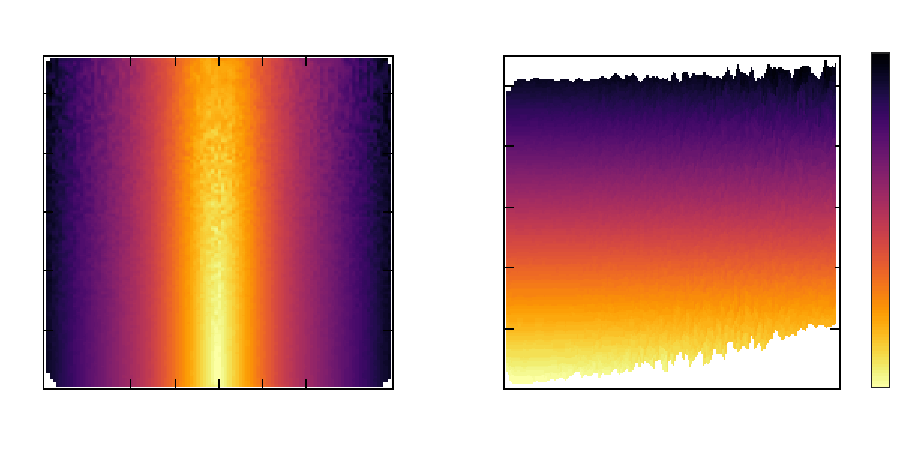
\includegraphics[scale=0.6]{./figures/slides/ch6/caer_x2}}%
    \gplfronttext
  \end{picture}%
\endgroup
